清华大学深圳研究生院紫荆志愿者服务团是清华大学深圳研究生院团委直属的学生志愿服务组织,以“自我实践、服务他人、自我教育、推动社会”为宗旨,旨在组织、协调我院研究生志愿者活动,开展具有清华特色的丰富多彩的研究生志愿活动。
\begin{figure}[!ht]
\centering
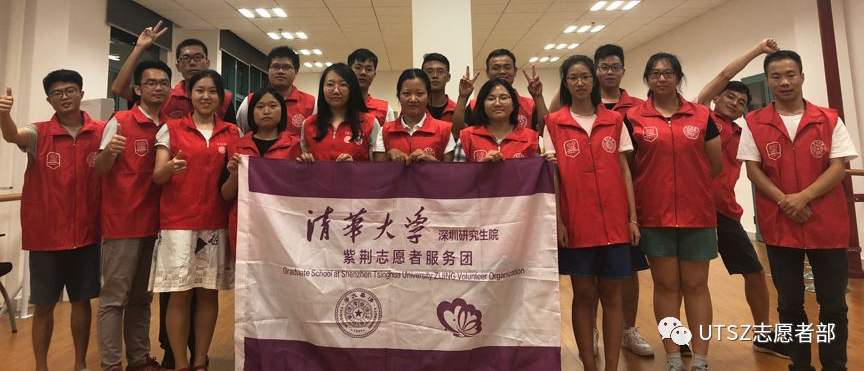
\includegraphics[width=14cm]{pic/zijing.png}
\end{figure}
2018年暑假,紫荆志愿团在海南省儋州市开展了支教扶贫系列活动,开拓了高校团队机器人支教的先河。


本次寒假清华大学深圳研究生院紫荆志愿者团拟开展的支教活动希望以成本价购入儿童机器人套装作为教具,发挥
自身专业优势开展支教活动。通过研究生寒假社会实践体系实现车费的报销。
%\begin{table}[!ht]
%\centering
%\begin{tabular}{|p{2cm}|p{2cm}|p{2cm}|p{3cm}|}
%\hline
%名称 & 来源 & 用途 \\
%\hline
%%深圳市搭搭乐乐文化传播有限公司
%儿童、初中机器人套装&  &  \\
%\hline
%素质拓展道具 & 心理辅导中心 &  \\
%\hline
%DOBOT魔术师(价值一万元) & 越疆科技 & \\
%\hline
%教具& &  \\
%\hline
%文具奖品 & & 课堂奖励 \\
%\hline
%\end{tabular}
%\caption{清华支教队所需教具参考}
%\end{table}

关于“旧洋关爱组”:旧洋村是一个支教点,紫荆团队和琼台师范学院2018年暑期在此支教。旧洋关爱组的实体是一个QQ群,由紫荆团队、琼台师范学院和支教地的孩子组成。各位支教老师利用自己的业余时间针对孩子暴露出的问题进行有针对性的疏导。紫荆团队在中秋佳节专程到东莞看望支教点的一个辍学的孩子,他现在跟着父母在莞城打工。
\begin{figure}[!ht]
\centering
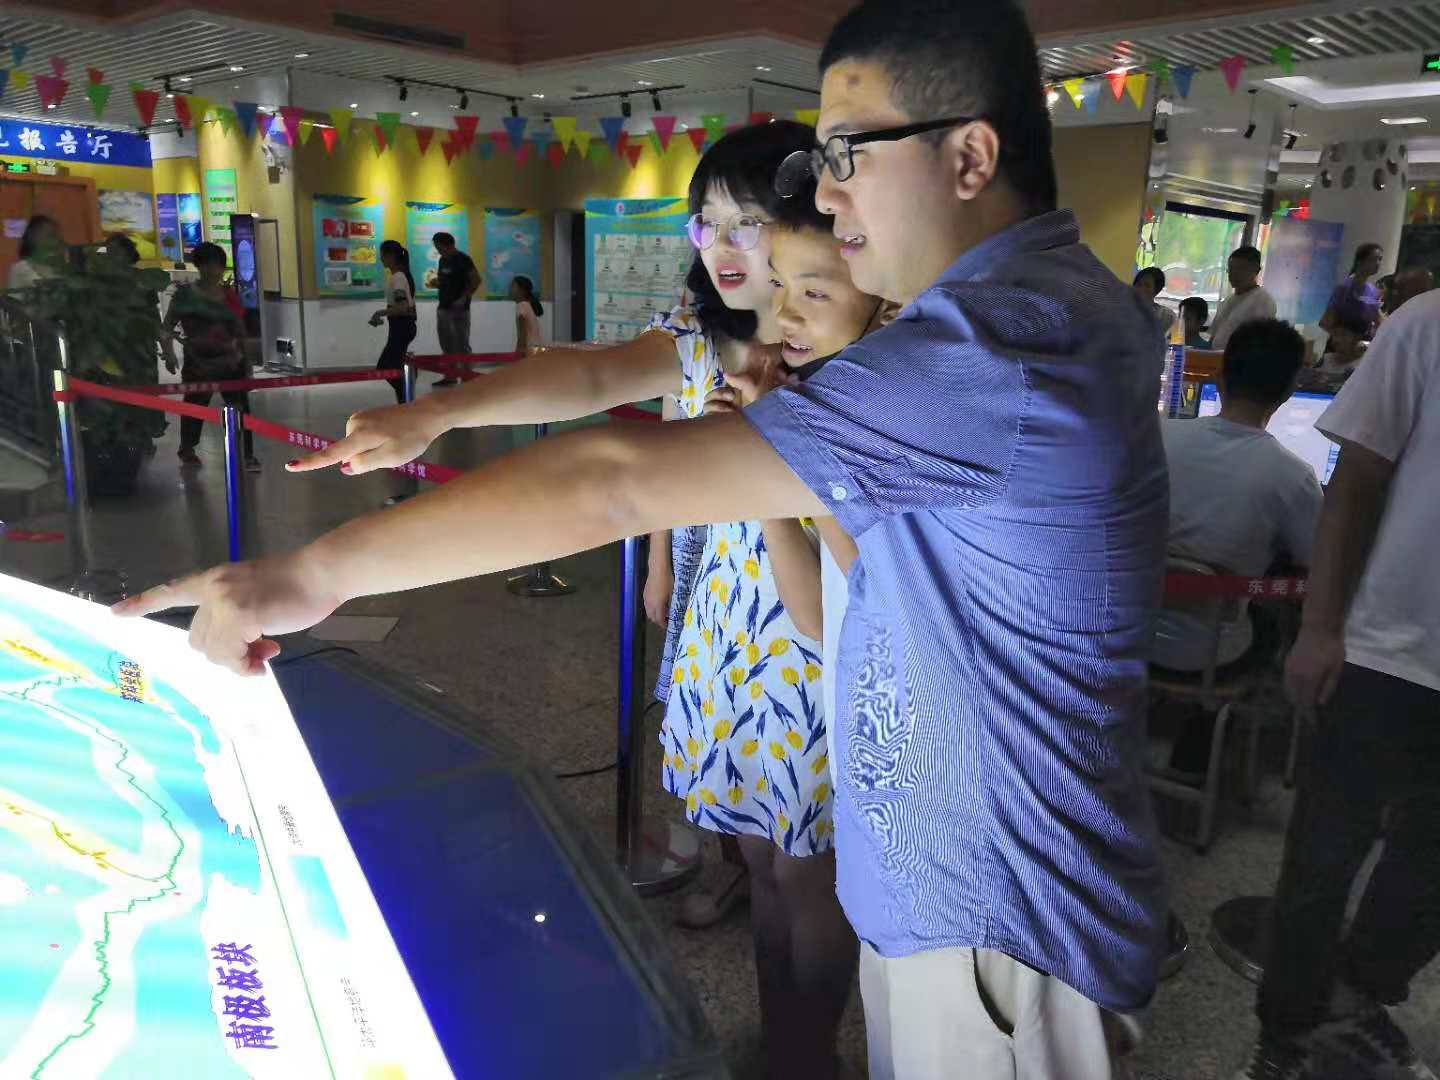
\includegraphics[width=12cm]{pic/zijing_talk.jpeg}
\caption{紫荆志愿者在东莞科技馆给孩子讲解}
\end{figure}